
%\newpage
%\pagenumbering{arabic}
MAYBE PUT SOME STUFF HERE ABOUT NUMERICAL ALGORITHMS LIKE RK4 EULAR STEP LEAPFROG AND DO ERROR GROWTH RATES AND COURANT


\section{Numerical Relativity}
\subsection{Spacetime Foliation}
Einstein's equation is a classical field equation which governs the dynamics of physical objects and spacetime curvature. 
\begin{equation}R_{\mu\nu} - \frac{1}{2} Rg_{\mu\nu} = \frac{8\pi G}{c^4}T_{\mu\nu}\end{equation}
The above version is fully covariant, agnostic of the definition of time, and many solutions are known analytically, for instance Black Hole geometries. When the system of interest becomes more complicated, such as the case of orbiting objects which will be discussed later, finding an analytic expression becomes impossible. For low energy dynamics, Newtonian theory, Post-Newtonian theory and perturbation theory can make more progress; however this report will focus on the highly nonlinear regime where Numerical relativity is truly the only hope to solve Einstein's equations. To do this it is common to split spacetime into 3+1 dimensions, evolving a 3 dimensional manifold (maybe with matter) on a computer along the final 4th dimension. To do this we need to define a suitable hypersurface $\Sigma \in \M$. This is usually done by demanding the hypersurface $\Sigma_t$ be the set of points $p \in \M$ where some scalar function $f:\M\mapsto \mathbb{R}$ satisfies $f(p)=t$. This hypersurface should be a Cauchy surface, intersecting all causal curves only once, or a partial Cauchy surface which intersects all causal curves at most once. Generally we will choose a partial Cauchy surface due to the finite memory of computers, however by picking certain compactified coordinates it is possible to use a Cauchy surface [ref]. A foliation $\mathcal{F}$ is then the union of a set of $\Sigma_t$ for some range of the parameter $t$.
\[\mathcal{F} = \cup_t(\Sigma_t) \subseteq \M\]
This means we should be careful to pick a parameter $t$ such that the foliation is not self intersecting for the parameter range that covers the region of $\M$ that we are interested in simulating. Fortunately the time coordinate in a suitable coordinate system works in all cases covered by this report; it also gives the physical interpretation of $\Sigma_t$ being an instance of time. Now we should define unit normal vector $n$ to $\Sigma_t$.
\begin{equation} n^\mu = -\frac{\nabla^\mu t}{\sqrt{|g_{\mu\nu}\nabla^\mu t \nabla^\nu t|}} \quad \& \quad  n_\mu = -\frac{dt_\mu}{\sqrt{|g_{\mu\nu}\nabla^\mu t \nabla^\nu t|}}\end{equation}
For simplicity we define the lapse function $\alpha$ to be
\begin{equation}\alpha :=  \frac{1}{\sqrt{|g_{\mu\nu}\nabla^\mu t \nabla^\nu t|}} \end{equation}
giving us $n_\mu = -\alpha \dd t_\mu$ as well as the normal evolution vector $m_\mu = \alpha n_\mu$. Defining two infinitessimaly close points $(p,q)\in(\Sigma_t,\Sigma_{t'})$ where $ q^\mu = p^\mu + m^\mu\delta t$ we see
\[ t(q) = t(p^\mu +  m^\mu\delta t) = t(p) + \frac{\dd t}{\dd x^\mu}m^\mu\delta t = t(p) + \dd t_\mu m^\mu \delta t =  t(p) + \delta t\] 
showing that $m^\mu$ points between neighbouring hypersurfaces; therefore when creating evolution equations we should care about Lie derivates along $m^\mu$, $\L_m$, rather than $\L_n$.



\subsection{The 3+1 Decomposition}
With the notion of a spacetime foliation we should define how to project tensors onto $\Sigma_t$; clearly scalars need no projecting. Splitting a vector $X^\mu e_\mu = X^\mu_\| e_\mu + X^\mu_\perp e_\mu$ into components tangent or normal to $\Sigma_t$ we define the orthogonal projector $\perp^\mu_\nu$ and parallel projector $-n^\mu n_\nu$.
\begin{align}X^\mu_\| &= \left[ \delta^\mu_\nu + n^\mu n_\nu\right] X^\mu  = \perp^\mu_\nu X^\nu\\
X^\mu_\perp &= -n^\mu n_\nu X^\nu \end{align}
Considering scalars such as $\phi = w_\mu X^\mu$ or $\psi = T^{\mu\nu}w_\mu w_\nu$, and remembering scalars don't vary under projection, it is simple to show that any tensor $T$ can be projected by contracting a projection operator $\perp$ on any free index.
\begin{equation} {T_\|}^{ab ...}_{\;\;\;\;\;\;\;cd ...} = {\mathcal{T}}^{ab ...}_{\;\;\;\;\;\;\;cd ...} =\perp^{a}_{A}\perp^{b}_{B}\perp^{C}_{c}\perp^{D}_{d}\cdot\cdot\cdot\, T^{AB ...}_{\;\;\;\;\;\;\;\;\;\;CD ...}\end{equation}
We can find the 3 metric $\gamma_{\mu\nu}$ of $\Sigma_t$ by projecting $g_{\mu\nu}$ 
\begin{equation} \gamma_{ij} = \perp^\mu_i \perp^\nu_j g_{\mu\nu} = g_{\mu\nu} + n_\mu n_\nu\quad \rightarrow \quad \gamma^i_j = \perp^i_j\end{equation}
and we find it is equivalent to the projector $\perp$; this had to be the case as $\perp_{ij}\dd x^i\dd x^j$ gives the line element along $\Sigma_t$. With this machinery we can define the extrinsic curvature tensor $\K_{ij}$ representing curvature due to the choice of spacetime foliation; it could be nonzero for certain foliations of Minkowski space. It is not the same as the 3-Ricci tensor $\R_{ij}$ which is due to genuine spacetime curvature of $\M$ regardless of foliation. The extrinsic curvature tensor is defined the following way
\begin{align} \K_{ij}  &= \K_{ji}:= -\perp_i^\mu \perp_j^\nu \nabla_\mu n_\nu = -\perp_i^\mu \nabla_\mu n_j = -\nabla_i n_j - n_i a_j \\
\K &= \K_i^i = -\nabla \cdot n\end{align}
where $a_i = n\cdot\nabla n_i $ is called the Eularian acceleration; it should be noted $\K_{ij}$ is symmetric. It can also be shown to take the following form
\begin{equation} \K_{ij} = -\frac{1}{2}\L_n \gamma_{ij} = -\frac{1}{2\alpha}\L_m \gamma_{ij}\end{equation}
which gives the intuitive explanation of $\K_{ij}$ being the rate of change of the 3-metric $\gamma_{ij}$ with respect to the foliation. 
The next object we should discuss is the projected covariant 3-derivative $\D_i$. This is the covariant derivative belonging to $\Sigma_t$ and hence it's arguments should be tensors belonging to $\Sigma_t$. This means we can define it as so
\begin{align} {{T}}^{ab ...}_{\;\;\;\;\;\;\;cd ...} &=  \perp^{a}_{A}\perp^{b}_{B}\perp^{C}_{c}\perp^{D}_{d}\cdot\cdot\cdot\, T^{AB ...}_{\;\;\;\;\;\;\;\;\;\;CD ...},\\
  \D_\mu {{\mathcal{T}}}^{ab ...}_{\;\;\;\;\;\;\;cd ...} :&=   \perp^\nu_\mu  \perp^{a}_{A}\perp^{b}_{B}\perp^{C}_{c}\perp^{D}_{d} \nabla_\nu{\mathcal{T}}^{AB ...}_{\;\;\;\;\;\;\;\;\;\;CD ...}.\end{align}
A simple example is the derivative of a vector $X^i e_i \in \T(\Sigma_t)$
\begin{gather} \D_i X^j = \partial_i X^j + \Upsilon^i_{\;\,jk}X^k\nonumber\\
\Upsilon^i_{\;\,jk} = \frac{1}{2}\gamma^{il}\left[ \partial_{j}\gamma_{lk} + \partial_{k}\gamma_{jk} -\partial_{l}\gamma_{jk} \right]\end{gather}
where $\Upsilon^i_{\;\,jk}$ is the Christoffel symbol of $\Sigma_t$. Another useful example is $a^\mu$ which can be equated to
\[ a_\mu = n\cdot \nabla n_\mu = \D_\mu \ln \alpha = \frac{1}{\alpha}\D_\mu \alpha\]
and allows us to evaluate the Lie derivative of the projector $\perp^i_j$.
\begin{gather*}\L_m \perp^i_j = \alpha n^k \nabla_k \perp^i_j + \perp^i_k \nabla_j \alpha n^k - \perp^k_j \nabla_k \alpha m^i  = \alpha n^k \nabla_k \left[ n^i n_j\right]  + \alpha \nabla_j n^i - \left[ \alpha K_j^i + n^i \D_j \alpha\right] = 0\end{gather*}
The result $\L_m \perp^i_j=0$ is incredibly important, it tells us that the projector commutes with $\L_m$ and as a result any tensor $T$ which when projected onto $\Sigma_t$, written $\T$, satisfies
\begin{equation}  \L_m {{\mathcal{T}}}^{ab ...}_{\;\;\;\;\;\;\;cd ...} =   \perp^{a}_{A}\perp^{b}_{B}\perp^{C}_{c}\perp^{D}_{d}\L_m{\mathcal{T}}^{AB ...}_{\;\;\;\;\;\;\;\;\;\;CD ...}.\end{equation} 
or in other words, evolving a projected tensor along integral curves of $m$ leaves the tensor parallel to $\Sigma_t$.




\subsection{Gauss, Codazzi and Ricci Equations}
We now have all the results we need to decompose the Riemann and Ricci tensors and scalar. From the definition of the Riemann tensor we know
\begin{gather*} [\mathcal{D}_\alpha\mathcal{D}_\beta-\mathcal{D}_\beta\mathcal{D}_\alpha]v^\gamma = \mathcal{R}^\gamma_{\,\,\,\lambda \alpha\beta}v^\lambda, \\
 [\nabla_\alpha\nabla_\beta-\nabla_\beta\nabla_\alpha]v^\gamma = {R}^\gamma_{\,\,\,\lambda \alpha\beta}v^\lambda, \end{gather*}
where the vector $v^\lambda = \perp^\lambda_\rho v^\rho$ is tangent to $\Sigma_t$. Expanding the $\mathcal{D}$'s into $\nabla$'s gives
\[ \mathcal{D}_\alpha \mathcal{D}_\beta v^\gamma = \perp^\mu_\alpha \perp_\beta^\sigma \perp^\gamma_\xi \nabla_\mu(\perp^\nu_\sigma \perp^\xi_\rho \nabla_\nu v^\rho)\]
and using the following properties; impotence of projections $\perp^\alpha_\mu \perp^\mu_\beta = \perp^\alpha_\beta$, null projection of orthogonal vectors $\perp n =0$, metric compatibility $\nabla_\mu \perp^\alpha_\beta = n_\beta\nabla_\mu n^\alpha + n^\alpha \nabla_\mu n_\beta$ and equation () for $\K_{ij}$ we obtain the Gauss relation.
\begin{equation} \perp^\mu_\alpha \perp^\nu_\beta \perp^\gamma_\rho \perp^\sigma_\delta R^{\rho}_{\,\,\,\sigma\mu\nu} = \mathcal{R}^\gamma_{\,\,\,\delta\alpha\beta} + \mathcal{K}^\gamma_\alpha \mathcal{K}_{\delta\beta} - \mathcal{K}^\gamma_\beta \mathcal{K}_{\alpha\delta}  \end{equation}
Contracting over $\alpha,\gamma$ above and relabelling indices we get the contracted Gauss relation.
\begin{equation} \perp^\mu_\alpha \perp^\nu_\beta R_{\mu\nu} + \gamma_{\alpha\mu}n^\nu\perp^\rho_\beta n^\sigma R^\mu_{\,\,\,\nu\rho\sigma} = \mathcal{R}_{\alpha\beta} + \mathcal{K} \mathcal{K}_{\alpha\beta} - \mathcal{K}^\mu_\beta \mathcal{K}_{\alpha\mu}  \end{equation}
Contracting again and realising $R_{abcd}n^an^bn^cn^d=0$ from antisymmetry in indeces 0,1 or 2,3 in the Riemann tensor gives the scalar Gauss equation.
\begin{equation}R + 2R_{\mu\nu}n^\mu n^\nu = \mathcal{R} + \mathcal{K}^2 - \mathcal{K}_{\mu\nu}\mathcal{K}^{\mu\nu}\end{equation}
The Codazzi relations are derived from a different start point
$$  [\nabla_\alpha\nabla_\beta-\nabla_\beta\nabla_\alpha]n^\gamma = {R}^\gamma_{\,\,\,\lambda \alpha\beta}n^\lambda $$
and project down with 3 operators $\perp\perp\perp$. The following relations are used 
\begin{gather*} \nabla_\beta n^\gamma = -\mathcal{K}^\gamma_{\,\,\,\beta} - a^\gamma n_\beta,\\
 \perp^\alpha_\mu \perp^\beta_\nu \perp^\rho_\gamma \nabla_\alpha \nabla_\beta n^\gamma = -\mathcal{D}_\alpha \mathcal{K}^\gamma_{\,\,\,\beta} + a^\gamma \mathcal{K}_{\alpha\beta},\end{gather*}
which lead immediately to the Codazzi relation
\begin{equation}\perp_\alpha^\mu \perp_\beta^\nu \perp^\gamma_\rho n^\sigma R^\rho_{\,\,\,\sigma\mu\nu} =  \mathcal{D}_\beta \mathcal{K}^\gamma_{\,\,\,\alpha} -\mathcal{D}_\alpha \mathcal{K}^\gamma_{\,\,\,\beta}\end{equation}
and the contracted Codazzi relation.
\begin{equation}\perp^\mu_\alpha  n^\nu R_{\mu\nu} =  \mathcal{D}_\alpha \mathcal{K} -\mathcal{D}_\mu \mathcal{K}^\mu_{\,\,\,\alpha}\end{equation}

Finally we turn our attention to the Ricci equation. We start with the Riemann term in the contracted Gauss equation,
\[\gamma_{\alpha\mu}\perp^\rho_\beta n^\sigma R^\mu_{\,\,\,\nu\rho\sigma}n^\nu =
\gamma_{\alpha\mu}\perp^\rho_\beta n^\sigma\left[ \nabla_\rho\nabla_\sigma-\nabla_\sigma\nabla_\rho\right]n^\nu\]
and using the following two formulae with equation (D ln a)
\[ \nabla_\sigma n^\mu = -\mathcal{K}^\mu_{\,\,\,\sigma}-n^\mu \mathcal{D}_\sigma \ln(\alpha)\]
\[ \L_m \K_{ij}  = \perp^a_i\perp^b_j\L_m \K_{ab} =\perp^a_i\perp^b_j\left[ \alpha n\cdot \nabla \K_{ab} + 2 \K_{k(b}\nabla_{a)}m^k\right] \]
some algebra yields
$$  \gamma_{\alpha\mu}n^\sigma \gamma^\nu_\beta R^\mu_{\,\,\,\rho\nu\sigma} n^\rho = -\mathcal{K}_{\alpha\sigma}\mathcal{K}^\sigma_{\,\,\,\beta} +\frac{1}{\alpha}\mathcal{D}_\beta\mathcal{D}_\alpha \alpha + \gamma^\mu_\alpha\gamma^\nu_\beta n^\sigma \nabla_\sigma \mathcal{K}_{\mu\nu}.$$
From () we know $\mathcal{L}_m\mathcal{K}_{\alpha\beta} \in \Sigma_t$ and the projected Lie derivative is
$$  \mathcal{L}_m\mathcal{K}_{\alpha\beta} = \alpha \gamma^\mu_\alpha \gamma^\nu_\beta n^\sigma \nabla_\sigma \mathcal{K}_{\mu\nu} - 2\alpha\mathcal{K}_{\alpha\mu}\mathcal{K}^\mu_{\,\,\,\beta}.$$
This is what we need to derive the Ricci equation.
\begin{equation}\gamma_{\alpha\mu}n^\sigma \gamma^\nu_\beta R^\mu_{\,\,\,\rho\nu\sigma} = \frac{1}{\alpha}\mathcal{L}_m \mathcal{K}_{\alpha\beta} +\frac{1}{\alpha}\mathcal{D}_\beta\mathcal{D}_\alpha \alpha +\mathcal{K}_{\alpha\mu}\mathcal{K}^\mu_{\,\,\,\beta}  \end{equation}

\subsection{Decomposition of Einstein's Equation}
To evolve General Relativity numerically we must project the Einstein Equation into 3+1 dimensions. Relations between 3 and 4 dimensional geometric objects have been derived above and will be used to decompose the Einstein tensor $G_{\mu\nu}$ from the left hand side of (). The second component, for simulating non-vacumm spacetimes, is the 3+1 decomposition of the Stress tensor $T_{ab}$. We contract twice with $n$, then once with $n$ while projecting onto $\Sigma_t$ and finally twice projecting onto $\Sigma_t$ to get an energy, momentum and stress-like split.
\begin{align} \mathcal{E} &= T(n,n) = T_{ab}n^an^b\\
 \S_i &= -T(n,\cdot) = -\perp_i^a n^b T_{ab}\\
\S_{ij} &= \perp^a_i\perp^b_j T_{ab}\end{align}
By construction the following is true.
\[ T_{ab} = \mathcal{E} n_a n_b + \S_a n_b + \S_b n_a + \S_{ab}\]
With this and the Gauss-Codazzi equations () we can project the Einstein equation. Lets first look at the scalar equation
\[ G_{\mu\nu}n^\mu n^\nu = R_{\mu\nu}n^\mu n^\nu + \frac{1}{2}R = 8\pi \E\]
and equating the geometric terms to the scalar Gauss equation () we get the Hamiltonian constraint, $\mathcal{H}=0$.
\begin{equation}\mathcal{H} = \K_{\mu\nu}\K^{\mu\nu}-\K^2 -\R + 16\pi \E  \end{equation}
Now looking at the once projected part we see
\[ \perp^\mu_i n^\nu G_{\mu\nu} =  \perp^\mu_i n^\nu R_{\mu\nu} = -8\pi\S_i\]
and substituting the geometric terms for the contracted Codazzi relation we get the Momentum constraint, $\mathcal{P}_i = 0$.
\begin{equation} \mathcal{P}_i = \D_i \K - \D_j\K^j_i  + 8\pi \S_i\end{equation}
Finally, the space-space projection gives the 6 evolution PDE's. This time start with the trace reversed Einstein Equation
\begin{gather*} R_{\mu\nu} = 8 \pi \left[T_{\mu\nu} - \frac{1}{2}Tg_{\mu\nu}\right]\\
\perp^\mu_i\perp^\nu_jR_{\mu\nu} = 8 \pi \left[\S_{ij} - \frac{1}{2}T\gamma_{ij}\right]\\
T = \left[ \gamma^{\mu\nu} - n^\mu n^\nu\right]T_{\mu\nu} = \S-\E\end{gather*}
and to project the Ricci tensor, we use the contracted Gauss equation () but replace the term with $R^a_{\,\,\,bcd}$ with the Ricci equation (). Rearranging gives a normal evolution for the extrinsic curvature.
\begin{equation} \L_m \K_{ij} = -\D_j\D_i \alpha + \alpha \left[ \R_{ij} + \K\K_{ij} - 2\K^k_i\K_{kj} + 4\pi \left[ \gamma_{ij}\left[ \S-\E\right]-2\S_{ij}\right]\right]\end{equation}
Along with the definition of $\K_{ij}$ in equation (), this gives the normal evolution equations for $\gamma_{ij}$ and $\K_{ij}$. These contain 6 of the second derivatives in Einstein's equation, with the other 4 being the constraint equations to be satisfied along evolution.

\subsection{Foliation Adapted Coordinates, CHECK ERORR IN ADM METRIC MATRIX}
\begin{wrapfigure}{r}{0.65\textwidth}
    \includegraphics[width=0.65\textwidth]{adm.png}
\end{wrapfigure}
Picking coordinates in GR introudces a large gauge freedom, this allows us to use a level set of the time coordinate $x^0=t$ to define our foliation hypersurfaces $\Sigma_t$. The other three coordinates $x^i$ for $i\in[1,2,3]$ can be used to span each hypersurface $\Sigma_t$ however we define. It is conventional to split the normal evolution vector $m^\mu$ into time $t^\mu$ and space parts $\beta^\mu$.
\[ m^\mu = t^\mu - \beta^\mu  = (\partial_0)^\mu - \beta^i (\partial_i)^\mu \]
\[ m^\mu = \left( 1,-\beta^1,-\beta^2,-\beta^3\right) \]
We can view $t^\mu$ as the (not necessarily causal) worldline for a simulation gridpoint, hence we would like to evolve our PDE's along $t^\mu$ on a computer introducing advection terms like $\L_\beta$. Equations (def of m) specify $n^\mu$ and $n_\mu$
\begin{equation} n^\mu =  \frac{1}{\alpha}\left( 1,-\beta^1,-\beta^2,-\beta^3\right)\quad \& \quad n_\mu = -\alpha\left( 1,0,0,0\right)\end{equation}
as well as the decomposed metric, using the property that $\beta$ is tangent to $\Sigma_t$ and orthogonal to $m$.
\begin{gather} g_{00} = g(\partial_0,\partial_0) = g(m + \beta^i \partial_i,m + \beta^j\partial_j) = g(m,m) + \beta^i \beta_j \langle \partial_i,\dd x^j \rangle = -\alpha^2 + \beta^i \beta_i \nonumber\\
 g_{0i} = \beta_i,\quad
 g_{ij} = g(\partial_i,\partial_j) = \gamma(\partial_i,\partial_j) = \gamma_{ij}\nonumber\end{gather}
This is commonly called the $3+1$ ADM metric and $\alpha$, $\beta^i$ are referred to the lapse and shift vector in this context. The metric is commonly written as follows.
\begin{gather}\dd s^2 = -\alpha^2 \dd t^2 + \gamma_{ij}\left[\dd x^i + \beta^i \dd t\right]\left[\dd x^j + \beta^j \dd t\right]\\
 g_{\mu\nu} = \begin{pmatrix} -\alpha^2 + \beta^i \beta_i & \beta_i \\ \beta_j & \gamma_{ij} \end{pmatrix}\quad \leftrightarrow\quad g^{\mu\nu} = \begin{pmatrix} -\alpha^{-2}  & -\alpha^{-2} \beta^i \\ -\alpha^{-2}\beta^j & \gamma^{ij} - \alpha^{-2}\beta^i \beta^j \end{pmatrix}\end{gather}
and using Cramers rule for metric determinant
\[ g^{00} = \frac{\det{\gamma_{ij}}}{\det{g_{\mu\nu}}}\]
we get the important relationship
\begin{equation} \sqrt{-g} = \alpha \sqrt{\gamma} .\end{equation}

\subsection{ADM Equations}
Now that we have some coordinates suitable for the spacetime foliation we can find the ADM evolution equations for $\K_{ij}$ and $\gamma_{ij}$. First expand the Lie derivative $\L_m$ using
\[ t^{\mu} = (1,0,0,0) \rightarrow \L_t {{T}}^{ab ...}_{\;\;\;\;\;\;\;cd ...} = \partial_t {{T}}^{ab ...}_{\;\;\;\;\;\;\;cd ...}\]
\[ \L_m = \L_{t} - \L_\beta  = \partial_t - \L_\beta\]
and the ADM equations can be written by expanding the $\L_m$ in equations (). 
\begin{align} \partial_t \K_{ij} &= \L_\beta \K_{ij}  -\D_j\D_i \alpha + \alpha \left[ \R_{ij} + \K\K_{ij} - 2\K^k_i\K_{kj} + 4\pi \left[ \gamma_{ij}\left[ \S-\E\right]-2\S_{ij}\right]\right]\\
\partial_t \gamma_{ij} &= \L_\beta \gamma_{ij} - 2\alpha\K_{ij}\end{align}
Unfortunately, these PDE's turn out to be ill-posed []; the resolution comes in the next section.


\subsection{BSSN}
To tackle the ill-posedness of the ADM equations () the Baumgarte-Shapiro-Shibata-Nakamura (BSSN) formalism is introduced []. Another strongly hyperbolic formalism is the generalised harmonic gauge \cite{harmonic} with $ \Box x^\mu = H^\mu$. The first step in BSSN is to decompose the 3-metric into the conformal metric $\tilde{\gamma}_{ij}$ and the conformal factor $\chi$
\begin{equation} \tilde{\gamma}_{ij} = \chi \gamma_{ij}\quad\rightarrow\quad \det{\tilde{\gamma}_{ij}} = \tilde{\gamma} = \chi^3\gamma = 1\end{equation}
with the above being the convention used in GRChombo; other conventions include factors such as
\[  \tilde{\gamma}_{ij} = \psi^{-4}\gamma_{ij} \quad \mathrm{or} \quad e^{-\phi}\gamma_{ij}.\]
 Along with this the extrinsic curvature $\K_{ij}$ is modified to be trace free, $\A_{ij}$.
\[ \tilde{A}_{ij} = \chi\left[ \K_{ij}-\frac{1}{3}\K\gamma_{ij}\right]\quad\rightarrow \quad\tilde{A}_{ij}\gamma^{ij}=0\]
During an evolution the conditions $\trace{\tilde{A}_{ij}=0}$  and $\tilde{\gamma}=1$ are enforced which are observed to improve numerical stability; however it is unclear why beyond heuristic arguments. The definition of $\chi = \gamma^{-1/3}$ is good for black hole simulations where $\gamma\rightarrow\infty$ but $\chi \rightarrow 0$; for example the isotropic schwarzschild metric has \[\gamma = \left[ 1+ \frac{M}{2r}\right]^{12}\quad \rightarrow \quad \chi =\left[ \frac{r}{\frac{M}{2} + r}\right]^4.\] 
The next step is to introduce the conformal connection functions as auxiliary variables. 
\begin{align} \tilde{\Upsilon}^i &= \tilde{\gamma}^{jk}\tilde{\Upsilon}^i_{\,\;jk} = -\partial_i \tilde{\gamma}^{ij}\\
 \tilde{\Upsilon}^i_{\,\;jk} &= \frac{1}{2}\tilde{\gamma}^{il}\left[ \partial_j \tilde{\gamma}_{kl} + \partial_k \tilde{\gamma}_{lj} - \partial_l \tilde{\gamma}_{jk}\right] = \Upsilon^i_{\;\,jk} + \left[ \delta^i_j \partial_k + \delta^i_k \partial_j - \gamma^{il}\gamma_{jk}\partial_l\right] \ln \sqrt{\chi}\end{align}
Promoting these to evolution variables changes the hyperbolicity of the characteristic matrix and make the system well posed. This reduces the set of vacuum evolution variables to $\{\chi,\tilde{\gamma}_{ij},\K,\tilde{\A}_{ij},\tilde{\Upsilon}^i \}$. It is conventional to use $-\partial_i \tilde{\gamma}^{ij}$ to evaluate the conformal connection coefficients when they appear in the RHS of an equation, but $\partial_j \tilde{\Upsilon}^i$ is calculated by differentiating the evolution variable $\tilde{\Upsilon}^i$. One final detail, not included in the CCZ4 formulation discussed later, is to add multiples of the constraints () to the evolution equations to change the characteristic matrix and improve stability.


\subsection{Z4 Formalism}
The Z4 formalism \cite{z4} generalises the Einstein equation () to include an unphysical field $Z_\mu$, along with damping terms parameterised by $\kappa_1$, $\kappa_2$. 
\begin{equation} R_{\mu\nu} + \nabla_\mu Z_\nu + \nabla_\nu Z_\mu - \kappa_1\left[ n_\mu Z_\nu + n_\nu Z_\mu - [1+\kappa_2]g_{\mu\nu}n^\alpha Z_\alpha\right] = 8\pi G \left[T_{\mu\nu}- \frac{1}{2}Tg_{\mu\nu} \right]\end{equation}
Of course regular General Relativity is returned setting $Z_\mu=0$. It is shown in [] that achieving $Z_\mu=0$ whilst dynamically evolving $Z_\mu$  is equivalent to solving the constraints. $Z_\mu$ is subjected to a wave equation, transporting constraint violation off the computational domain. It can be shown that the system is driven to $Z_\mu =0$ for $k_1>0$ and $k_2<-1$. It is much cheaper to evolve the variables $Z_\mu$, driven to zero, than do perform four elliptic solves for the constraints $\{\mathcal{H},\M^i\}$ on each timestep. 

\subsection{CCZ4}
Joining BSSN with Z4 gives the CCZ4 formalism. The additional modifications
\begin{align} \Theta &= -n\cdot Z  = -\alpha Z^0\\
\hat{\Upsilon}^i &= \tilde{\Upsilon}^i + \frac{2\gamma^{ij}Z_j}{\chi}\end{align}
are made, leaving us with the following set of vacuum evolution variables $\{\chi, \tilde{\gamma}_{ij},\K,\tilde{\A}_{ij},\hat{\Upsilon}^i,\Theta \}$. Notably the pair of variables $\R_{ij} + \D_{(i}Z_{j)}$, and traced version $\R + \D\cdot Z$, always appear together; separately they ruin strong hyperbolically but together they do not. The Evolution equations can now be found in the CCZ4 scheme using the following equations (list evolution equations and decomposition of $\Upsilon$). Note the last two equations () are for the 3+1 Klein-Gordon equation which will be derived later in (). 
\begin{align} \partial_t \chi &=  \beta^k \partial_k \chi + \frac{2\chi}{3} \left[\alpha \K - \partial_k \beta^k \right]\\
\partial_t\tilde{\gamma}_{ij} &=  \beta^k\partial_k\tilde{\gamma}_{ij}  + \tilde{\gamma}_{kj}\partial_i \beta^k + \tilde{\gamma}_{ik}\partial_j\beta^k - \frac{2}{3}\tilde{\gamma}_{ij} \partial_k \beta^k - 2\alpha\tilde{\A}_{ij}\\
\partial_t\K &=  \beta^k\partial_k\K + \alpha\left[ \R + 2\D\cdot Z + \K\left[ \K-2\Theta\right]\right] - 3\alpha \kappa_1\left[ 1+\kappa_2\right]\Theta\\
&-\chi\tilde{\gamma}^{kl}\D_k\D_l\alpha + 4\pi G\alpha\left[ \S - 3\E\right]\nonumber \\
\partial_t\tilde{\A}_{ij} &=  \beta^k \partial_k \tilde{\A}_{ij}+\chi\left[\alpha\left[\R_{ij} + 2\D_{(i}Z_{j)}-8\pi G \S_{ij} \right] -\D_i\D_j\alpha \right]^{TF}\\
& +\tilde{\A}_{ij}\left[ \alpha\left[ \K-2\Theta\right]-\frac{2}{3}\K^2\right] + 2\tilde{\A}_{k(i}\partial_{j)}\beta^k -2\alpha\tilde{\gamma}^{kl}\tilde{\A}_{ik}\tilde{\A}_{lj}\nonumber\\
\partial_t\Theta &= \beta^k\partial_k \Theta + \frac{1}{2}\alpha\left[ \R + 2\D\cdot Z - \tilde{\A}_{kl} \tilde{\A}^{kl} + \frac{2}{3}\K^2 - 2\Theta\K\right] -\kappa_1\alpha\Theta\left[ 2+\kappa_2\right] - Z^k\partial_k\alpha - 8\pi G \alpha \E \\
\partial_t\hat{\Upsilon}^i &=  \beta^k \partial_k \hat{\Upsilon}^i + \frac{2}{3}\left[ \partial_k \beta^k \left[ \tilde{\Upsilon}^i+2\kappa_3 \frac{Z^{i}}{\chi}\right]-2\alpha\K\frac{Z^j}{\chi}\right]-2\alpha\kappa_1\frac{Z^i}{\chi}\\
& + 2\tilde{\gamma}^{ij}\left[ \alpha\partial_j\Theta -\Theta \partial_j\alpha \right] -2\tilde{\A}^{ij}\partial_j\alpha - \alpha\left[ \frac{4}{3}\tilde{\gamma}^{ij}\partial_j\K + 3\tilde{\A}^{ij}\frac{\partial_j \chi}{\chi}\right]\nonumber\\
& -\left[ \tilde{\Upsilon}^j + 2\kappa_3 \frac{Z^j}{\chi}\right]\partial_j \beta^i + 2\alpha \tilde{\Upsilon}^i_{\,\,\,jk}\tilde{\A}^{jk} + \tilde{\gamma}^{jk}\partial_j\partial_k \beta^i + \frac{1}{3} \tilde{\gamma}^{ij}\partial_k \partial_j \beta^k - 16\pi G \alpha \tilde{\gamma}^{ij}\S_j\nonumber\\
\partial_t \vp &= \beta^k\partial_k \vp - \alpha\Pi\\
\partial_t \Pi &= \beta^k\partial_k\Pi -\chi \tilde{\gamma}^{ij}\partial_i \vp \partial_j \alpha + \alpha \left[ \chi \tilde{\Upsilon}^k\partial_k \vp+\frac{1}{2} \tilde{\gamma}^{lk}\partial_k\chi\partial_l\vp  - \chi \tilde{\gamma}^{ij}\partial_i \partial_j \vp + \K \Pi + V' \vp \right]\end{align}
Also used was the lie derivative for a tensor density $\T$ of weight $n$.\[ \L_X \T = \widetilde{\L}_X \T + n\T \partial_k X^k\]
Here $ \widetilde{\L}_X$ represents the differential operator that is equivalent to $\L_X$ if it didn't act on a tensor density. Also to be noted, in the CCZ4 equations there is an additional parameter $\kappa_3$ premultiplying terms in the evolution of $\hat{\Upsilon}^i$ which experimentally were found to ruin numerical stability for black hole simulations []. Setting $\kappa_3<1$ stabilises the simulation but at the cost of covariance. Later on it was realised that setting $\kappa_3=1$ and $\alpha\kappa_1\rightarrow\kappa_1$ retains covariance as well as numerical stability [].

The CCZ4 scheme proves useful in my simulations for a few reason. Firstly, any initial data that does not satisfy the constraints will not do so along evolution either when using BSSN. Given that superposition of solutions in GR does not generally give a new solution, but does approximate one for separated compact objects, all the simulated binaries considered in the report will have non constraint satisfying initial data. The boosted stars I use later are an exact solution of GR though, being a coordinate transformation from the exact resting soliton. The use of CCZ4 will help simulations satisfy the constraints even if they initially satisfy them; one reason being that finite resolution imposes some small deviation from the continuum solution. More importantly, the use of adaptive mesh refinement AMR introduces large interpolation errors into the simulation at the boundary of the different grid resolution levels. Finally, the Sommerfeld boundary conditions used are inexact in GR and will introduce small errors at the boundary that ruin constraint satisfaction. In all above cases, the CCZ4 system forces the evolution towards constraint satisfaction, despite the numerical errors and approximations.


\subsection{Gauge Conditions}
In GR, the lapse $\alpha$ and shift $\beta^i$ are freely specifiable being gauge variables, however they must be chosen carefully along with a suitable initial Cauchy surface $\Sigma_{t_0}$ for sensible foliations and numerical accuracy. Figure 1 (left) shows how a poor initial Cauchy surface could extend to the singularity for ingoing Eddington-Finkelstein coordinates; likely causing a simulation crash. In my work $\Sigma_{t_0}$ is chosen to be isotropic as in Figure 1 (right); not only does this allow trivial swapping between spherical polar and Cartesian (used in simulation) coordinates but also provides an initial Cauchy surface that's free of singularities and easy to compute. For a poor choice of lapse function, even a well chosen $\Sigma_{t_0}$ can advance to the singularity in finite simulation time.
  \begin{figure}[h]
  \caption{Penrose Diagrams, $\Sigma_{t_0}$ dashed, Left: Ingoing Eddington-Finkelstein Coordinates, Right: Isotropic Coordinates.}
  \centering
  \subfloat{\includegraphics[width=0.43\textwidth]{schwarzschild2.png}\label{fig:f1}}
  \hfill
  \subfloat{\includegraphics[width=0.5\textwidth]{schwarzschild.png}\label{fig:f2}}
\end{figure}

The simplest lapse choice would be to enforce $\alpha=1$, which is geodesic slicing, with the hypersurface following geodesics; given that geodesics can converge this can lead to hypersurface self-intersection which breaks the definition of a Cauchy surface and the simulation will likely fail. Another problem is that a black hole singularity can be reached in finite simulation time. This can be modified to the maximal slicing condition which keeps the volume element $\sqrt{-g}$ constant along geodesics. This means as $\gamma\rightarrow\infty$ nearing a singularity $\alpha\rightarrow0$ using equation (), causing the hypersurface to advance more slowly before a singularity is reached. This property is called singularity avoiding and is crucial for numerical stability (unless using excision?). 
%\begin{wrapfigure}{r}{0.4\textwidth}
 %   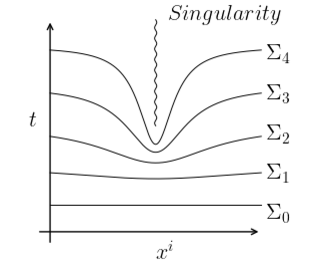
\includegraphics[width=0.4\textwidth]{foliation.png}
%\end{wrapfigure}
Maximal slicing can be implemented by forcing $\mathcal{K} = \partial_t \K = 0$ $\forall t$ which requires a slow elliptic solve for $\alpha$ at each timestep. Instead $\alpha$ is promoted to an evolution variable and is evolved along with every other simulation variable. To do this we can pick an algebraic slicing condition of the following type.
\[\L_m \alpha = -\alpha^2 f(\alpha)\K \]
This is used with $f = 2\alpha^{-1}$ in GRChombo giving
\[\L_m \alpha = -2\alpha \K \]
and using normal coordinates $\beta^i=0$ it reduces to 
\[ \alpha = 1+ \ln \gamma\]
which is called 1+log slicing; this is very common in Numerical Relativity codes. In practice 1+log slicing is strongly singularity avoiding reaching $\alpha=0$ before the singularity. This is modified in the CCZ4 scheme to 
\begin{equation}\partial_t \alpha = -2\alpha\left[ \K-2\Theta\right] + \beta^i \partial_i \alpha\end{equation}
which is very similar to before; it should be noted that the advection term is important for black hole simulations.

So far the shift vector $\beta^i$ has been ignored, the simplest choice for it would be $\beta^i=0$. Using 1+log slicing causes great stretching and shearing of $\Sigma_t$ in the neghbourhood of a singularity and choosing $\beta^i=0$ causes this shear to mean neighbouring gridpoints have large differences in field values leading to inaccurate and unstable evolutions. Another negative side effect is that the computational domain can fall inside an event horizon in black hole simulations. To counteract this we want to pick a shift vector that minimises hypersurface shear $\sigma_{ij}$ which can be defined as [ref 1977 smarr and york]
\[ \sigma_{ij}:= \perp^\mu_i \perp^\nu_j \left[\nabla_{(\mu} n_{\nu)}-\frac{1}{3}\gamma^{ab}\nabla_{(a} n_{b)} \gamma_{\mu\nu}\right] \]
where $\sigma_{ij}$ is tracefree corresponding to shearing rather than inflation or expansion. Minimising total shear, $\Sigma$,
\[ \Sigma = \int \sigma_{ij}\sigma^{ij}\sqrt{\gamma}\,\dd x^3\]
with respect to $\beta^i$ leads to an elliptic PDE to be solved for each $\beta^i$ at each time step that minimises shear. 
\[ \delta \Sigma = 0 \rightarrow \D_i\sigma^{ij}=0\]
This is known as the minimal shift condition. As before, promoting $\beta^i$ to be evolution variables is computationally cheaper. A very common choice is to promote the elliptic PDE for $\beta^i$ into a hyperbolic equation via introducing a $\partial_t^2\beta^i$ term and an artificial damping term parameterised by $\eta$. This becomes a damped wave equation and is supposed to transport away any part of $\beta^i$ which does not satisfy $\D_i \sigma^{ij}=0$. This requires Sommerfeld (outgoing wave) boundary conditions. In GRChombo the standard gamma driver shift condition is used.
\begin{align} \partial_t \beta^i &= FB^i\\
 \partial_t B^i &= \partial_t \tilde{\Gamma}^i - \eta B^i\end{align}
Here $F=3/4$ and $\eta=1$ are used in GRChombo.





